\section{Versuchsbeschreibung}

\subsection{Versuchsaufbau}

\begin{figure}[H]
	\centering 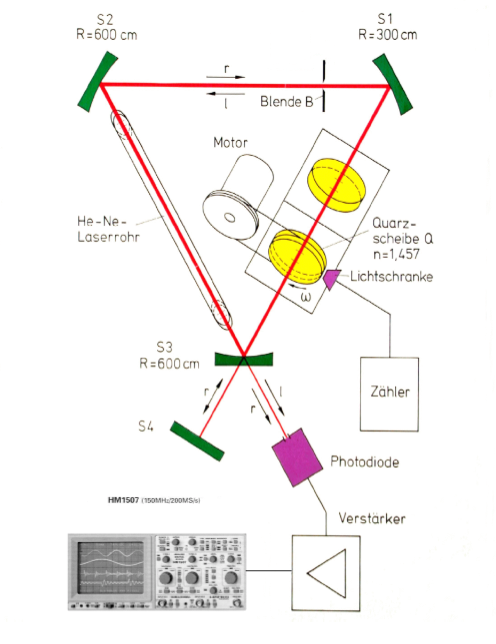
\includegraphics[width=0.6\textwidth]{Bilder/aufbau.jpg}
	\caption{Versuchsaufbau}
\end{figure}

\begin{figure}[H]
	\centering 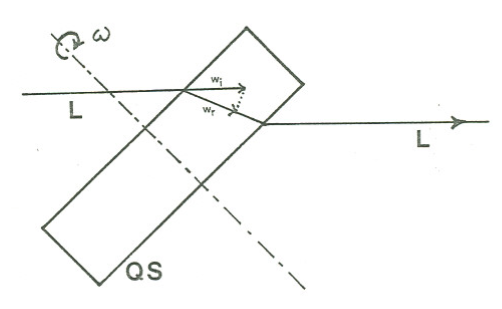
\includegraphics[width=0.6\textwidth]{Bilder/wiwr.jpg}
	\caption{Die Quarzscheibe}
\end{figure}

\subsection{Funktionsprinzip des Ringlasers}

Der Ringlaser ist ein dreieckiger Resonator, der aus 3 Spiegeln zusammengesetzt ist. In einem der drei Arme befindet sich ein He-Ne-Laser, der eine monochromatische, linear polarisierte Welle mit der Wellenlänge $6328.2 \ \mathring A$ in beide Richtungen in den Resonator abstrahlt. Somit läuft der eine Teil des Lichts links herum und der andere rechts herum (r-Strahl und l-Strahl). In einem zweiten Arm des Resonators befindet sich eine rotierende Quarzglasscheibe auf die der Laser unter dem Brewsterwinkel $\theta_B$ eintrifft, um Reflexionsverluste zu minimieren (siehe \emph{3.2. Der Brewserwinkel}). Durch die Rotation dieser Scheibe, wird das Licht innerhalb der Scheibe in die eine Richtung schneller, in die andere Richtung langsamer, jeweils um $+\alpha w_r$ oder $-\alpha w_r$. Hieraus folgt eine Änderung des optischen Weges und somit der optischen Länge des Resonators, sodass die Frequenzen in beide Richtungen erhöht bzw. erniedrigt werden. Hinter dem Auskoppelspiegel $S_3$ des Resonators interferieren diese Wellen dann und es entsteht eine Schwebung, aus der dann die Differenz der beiden Frequenzen ermittelt werden kann. Die zweite Quarzscheibe rotiert nicht und dient nur dazu den Versatz des Laserstrahls auszugleichen.